\section{Mechanism of On-Policy Distillation}
\label{sec:mechanism}

\Cref{sec:phenomenology} identified two conditions, thinking-pattern consistency and new knowledge beyond the same model family, that govern OPD effectiveness.
We now investigate the token-level mechanism through which these conditions manifest during training.
By comparing successful and failing OPD runs, we show that effective distillation is driven by progressive alignment on high-probability tokens.



\begin{tcolorbox}[takeawaysbox]
\begin{itemize}[topsep=0pt, partopsep=0pt, leftmargin=12pt, itemsep=0pt]
    \item \textbf{Progressive alignment.} The overlap between the student’s and teacher’s high-probability top-$k$ tokens increases steadily throughout training at student-visited states; failing runs show stagnant overlap from the outset.
    \item \textbf{Overlap sufficiency.} Nearly all of the optimization's effect concentrates on the shared top-$k$ tokens; optimizing only these overlap tokens suffices to match standard OPD, while non-overlap tokens contribute little.
\end{itemize}
\end{tcolorbox}

\subsection{Progressive Alignment of High-Probability Tokens}
\label{sec:alignment_high_prob}

We compare the dynamics of a single student distilled from two different teachers under the same settings, one yielding clear improvement and the other yielding none.
We find that successful OPD is essentially driven by learning the high-probability tokens shared between the student and teacher.

\paragraph{Setup.} We choose R1-Distill-1.5B as the student and compare two teachers: JustRL-1.5B and R1-Distill-7B.
The two teachers exhibit comparable math performance, with the latter being slightly stronger. We use the same DAPO-Math-17K dataset and training settings as before, and monitor three dynamic metrics during OPD.


\begin{figure*}[t]
    \centering
    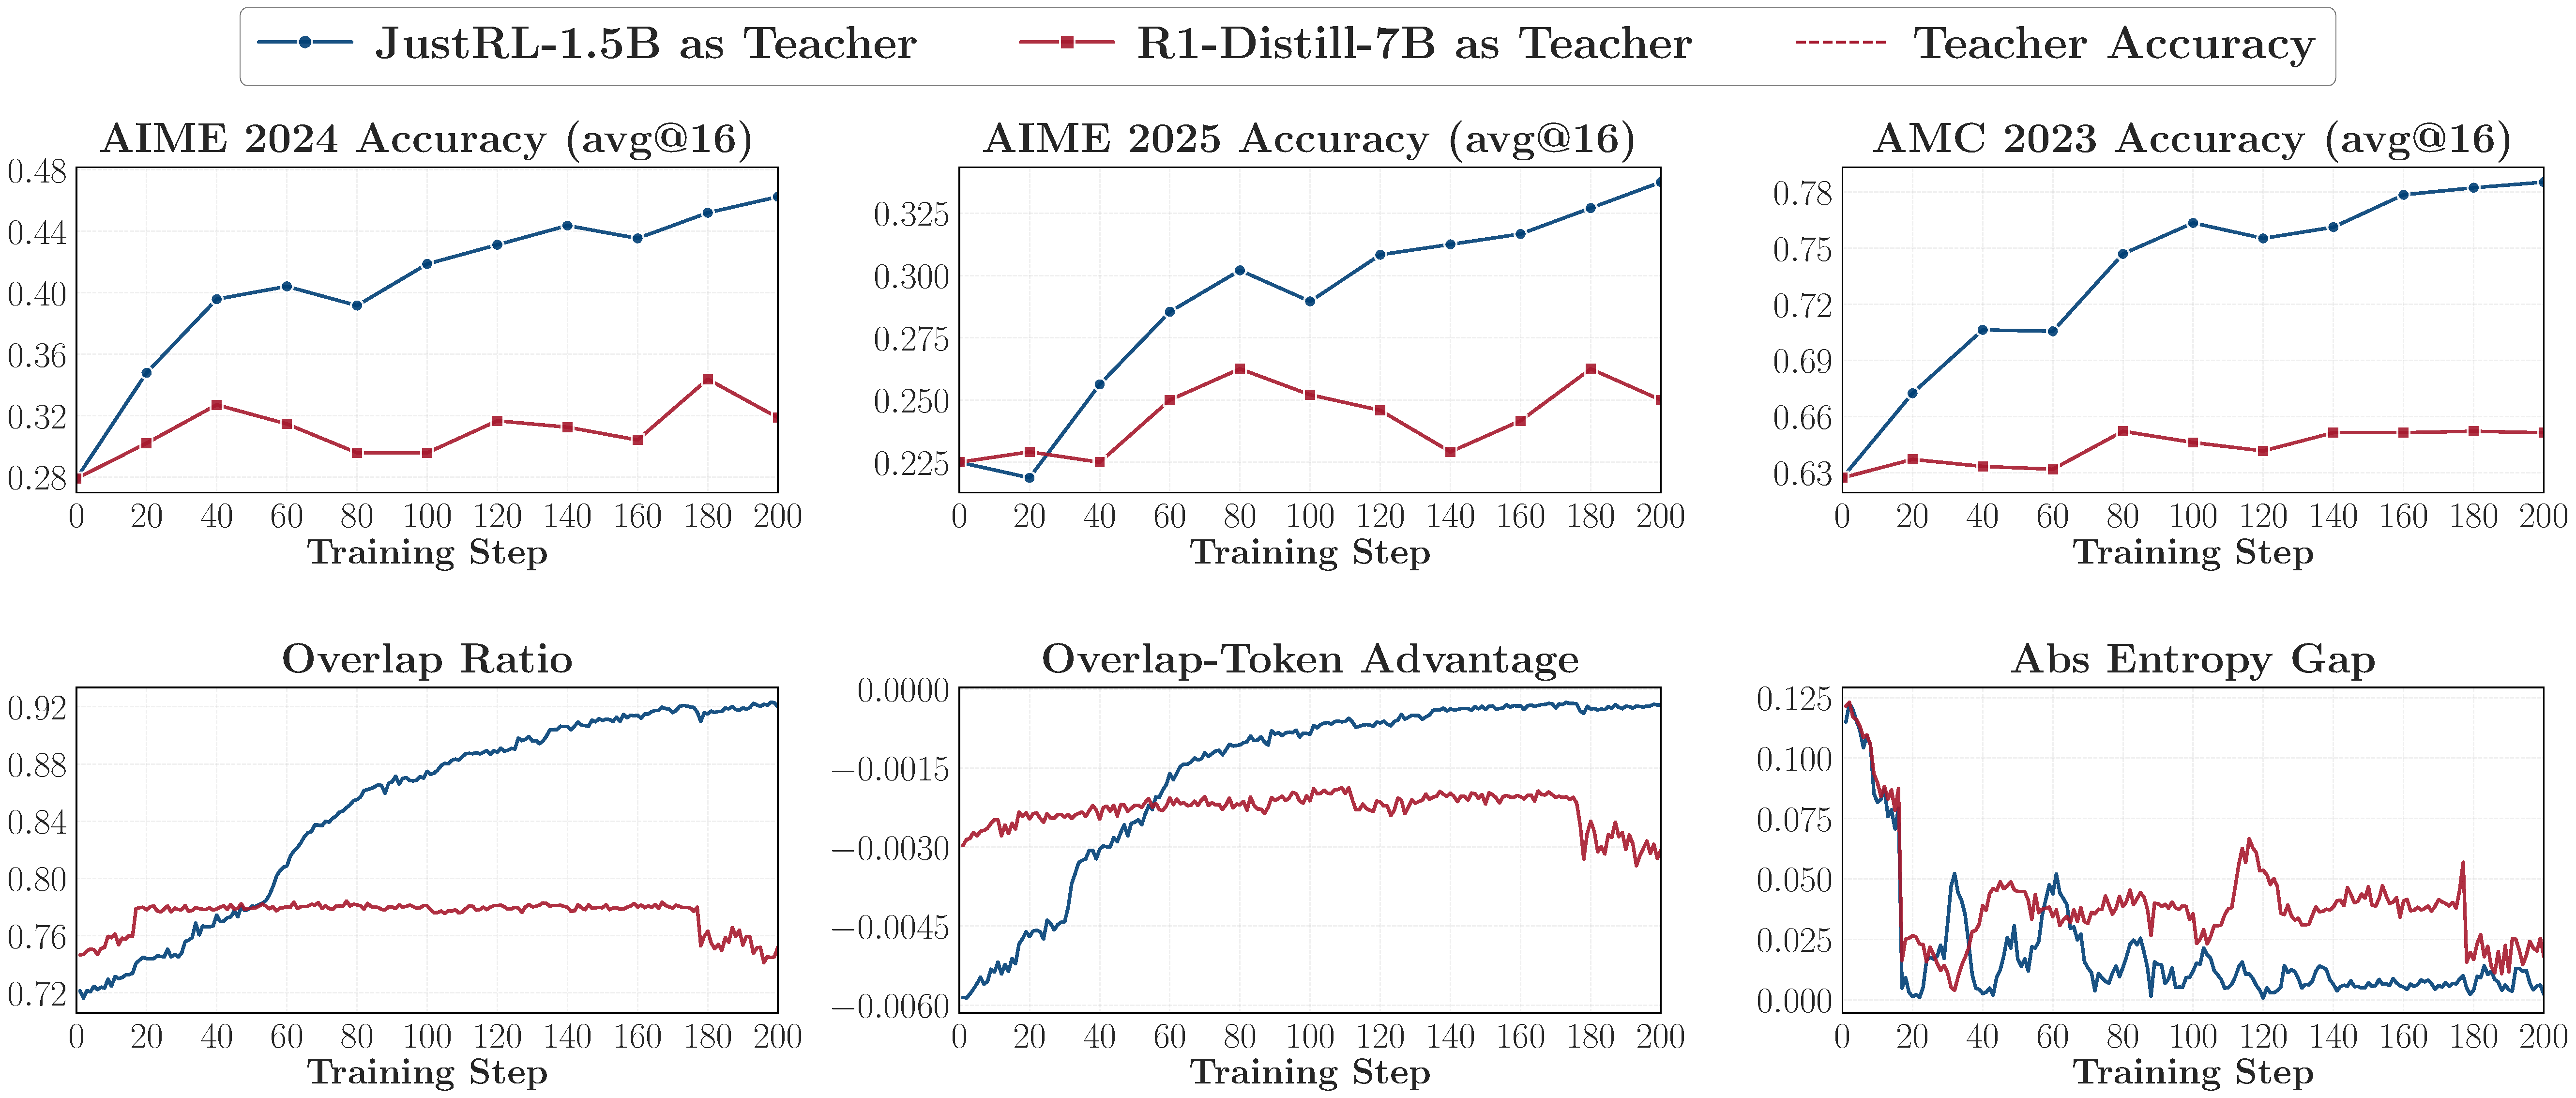
\includegraphics[width=\textwidth]{Figures/5.1/5_1_combined.pdf}
    \caption{
    Successful vs.\ failing OPD with the same student (R1-Distill-1.5B) and two teachers.
    \textbf{Top:} avg@16 accuracy on three benchmarks. Dashed lines indicate teacher performance.
    \textbf{Bottom:} three dynamics over training. Successful distillation (JustRL-1.5B) shows rising overlap and narrowing entropy gap, and these trends are absent in the failing run (R1-Distill-7B).
    }
    \label{fig:alignment_main}
\end{figure*}





\paragraph{Results.}
\Cref{fig:alignment_main} shows sharply different outcomes.
Distillation from JustRL-1.5B yields consistent gains, with the final student recovering more than $80\%$ of the performance gap to the teacher, whereas distillation from R1-Distill-7B fails to yield any improvement despite the teacher being stronger overall.
The training dynamics (\Cref{fig:alignment_main}, bottom) reveal the underlying divergence.
\textbf{In the successful run, the overlap ratio rises steadily, the overlap-token advantage improves toward zero, and the entropy gap narrows, indicating that the student progressively locates the teacher's high-probability region, calibrates its mass within that region, and matches the teacher's local confidence. In the failing run, all three metrics stagnate.}

Two observations deserve emphasis. First, the overlap tokens carry $97\%$-$99\%$ of the total probability mass for both models throughout training (see Appendix~\ref{app:overlap_mass}), so the rising overlap reflects alignment on the probabilistically dominant tokens, not merely a set-level coincidence.
Second, the improvement in overlap-token advantage suggests that OPD's primary optimization signal lies in reweighting probability within the overlap region rather than in tokens outside it.




We also report auxiliary optimization metrics (policy loss, gradient norm, and extreme-advantage token probability differences) in Appendix~\ref{app:auxiliary_dynamics}, which show consistent secondary patterns: the successful run exhibits decreasing loss and sustained gradient magnitude, while the failing run shows weak gradients and persistent probability discrepancies.
We further verify that these findings generalize across different model pairs in Appendix~\ref{app:cross_model_validation}, using R1-Distill-7B as the student with two different teachers under the same settings.






\vspace{-10pt}
\subsection{Optimizing Shared Tokens Alone Suffices}
\label{sec:overlap_enough}


The above analysis shows that high-probability token alignment correlates with OPD success.
We further investigate whether this correlation is causal: whether the overlap region is not only where alignment emerges, but also the region that drives optimization.
We design a targeted ablation that decomposes the top-$k$ support into its overlap and non-overlap parts, training on each in isolation.

\textbf{Setup.} Using the successful OPD setting from \Cref{sec:alignment_high_prob} (JustRL-1.5B $\to$ R1-Distill-1.5B), we compare three variants that differ only in which tokens the distillation loss covers: (i) \textbf{Student Top-$k$}, which optimizes on the full student top-$k$ support $S_t^{(p)}$; (ii) \textbf{Overlap Top-$k$}, which restricts optimization to the intersection of the student and teacher top-$k$ sets $S_t^{(p)} \cap S_t^{(q)}$; and (iii) \textbf{Non-Overlap Top-$k$}, which restricts optimization to their symmetric difference $S_t^{(p)} \triangle S_t^{(q)}$. We set default $k$ to $16$.



\begin{figure*}[t]
    \centering
    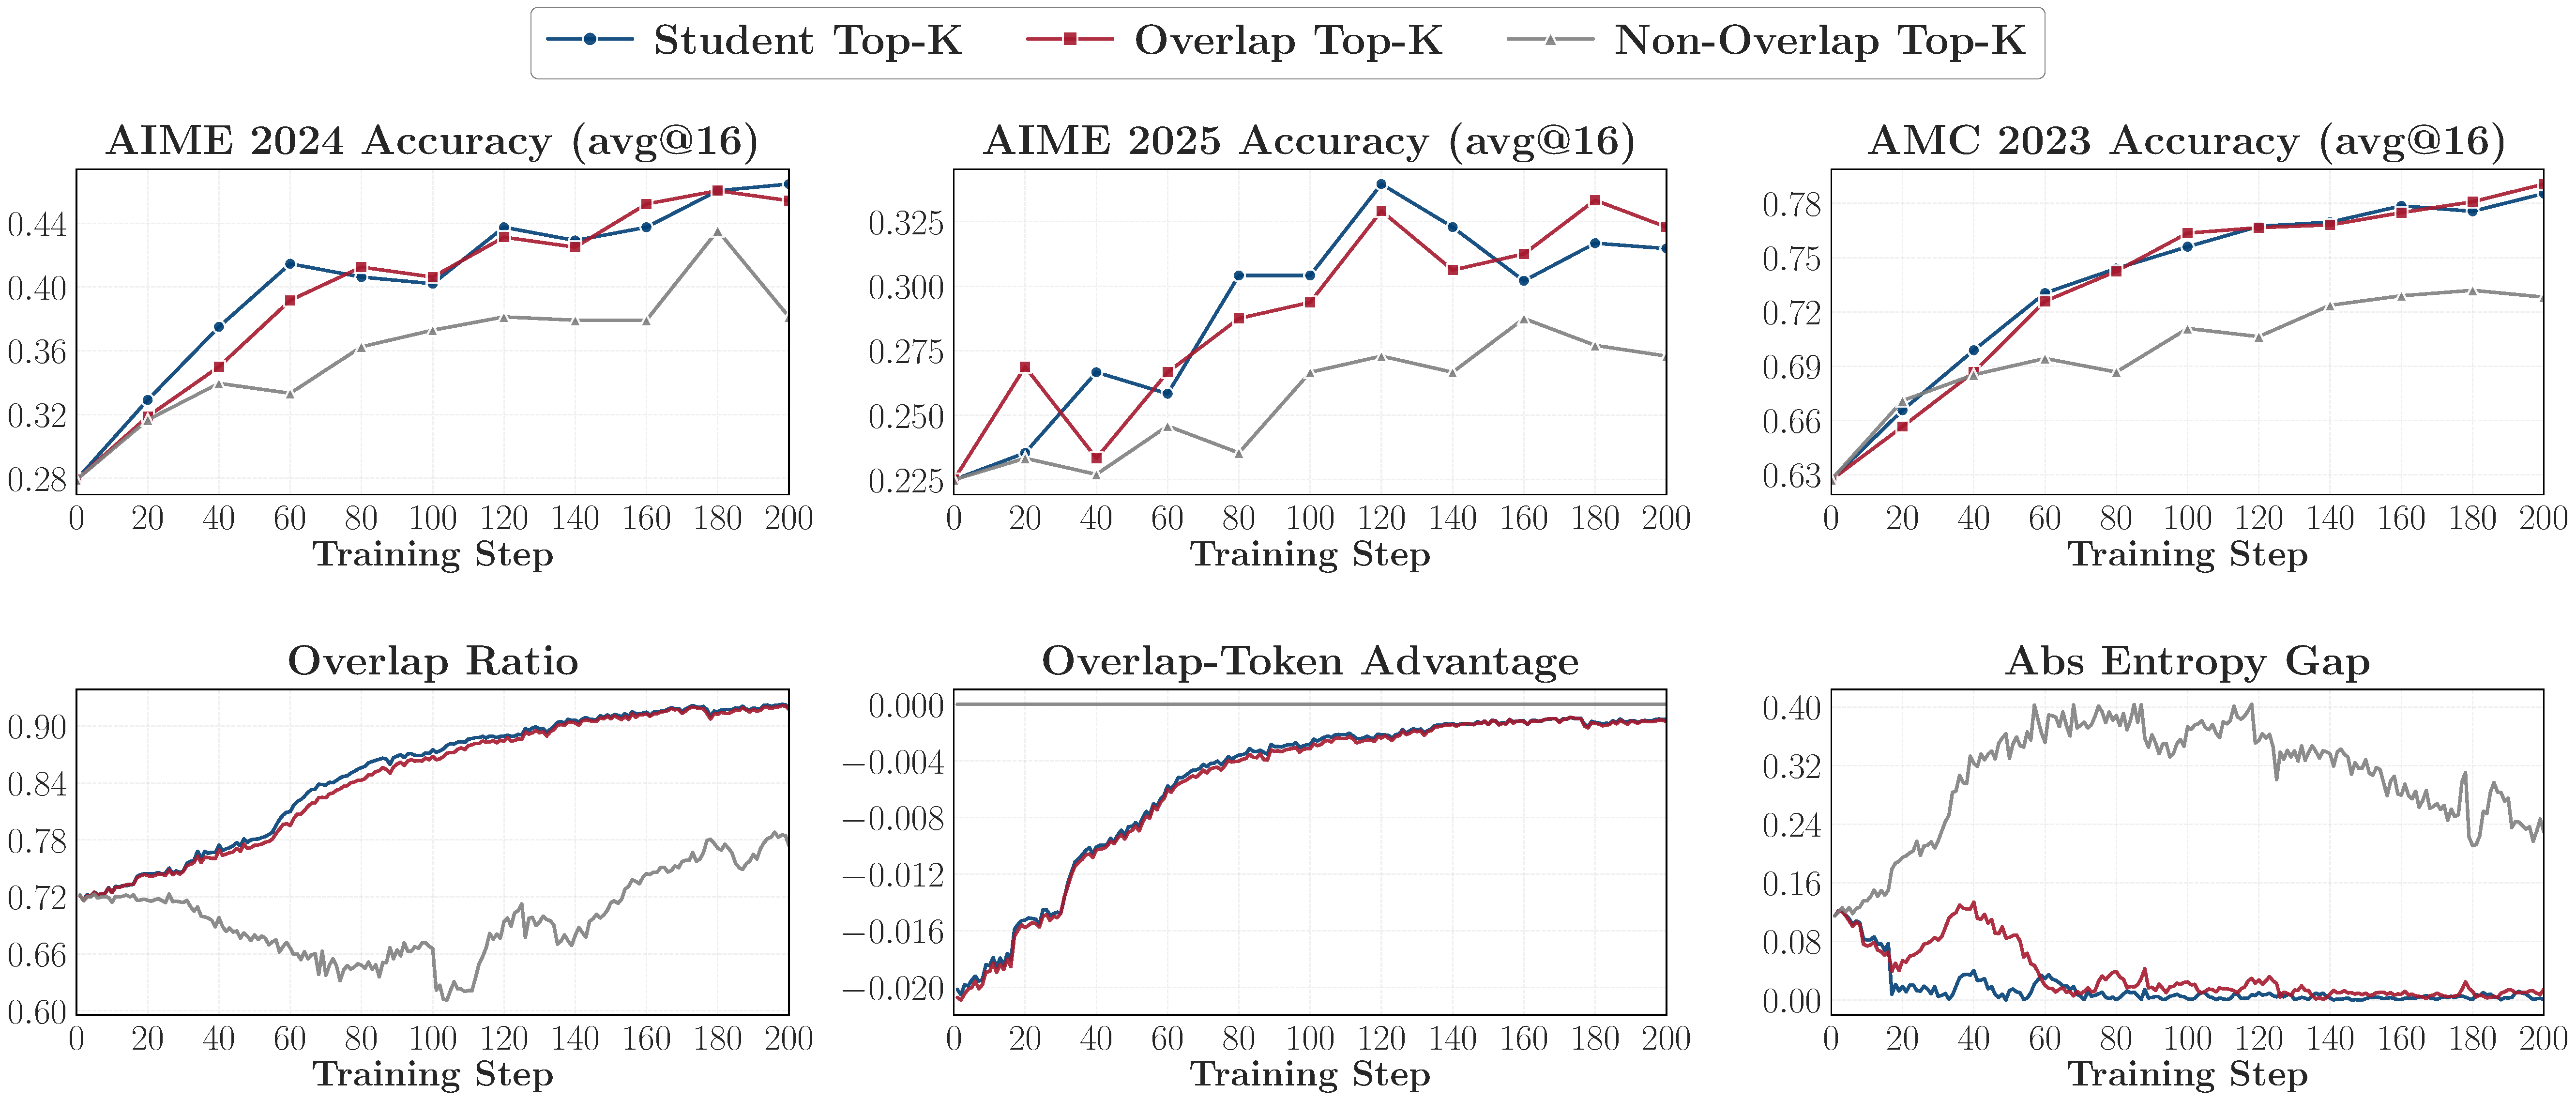
\includegraphics[width=\textwidth]{Figures/5.2/5_2_combined.pdf}
    \caption{
    Ablation on the optimization support in Top-$k$ OPD. Overlap Top-$k$ matches Student Top-$k$, while Non-Overlap Top-$k$ is substantially weaker.
    }
    \vspace{-4mm}
    \label{fig:overlap_enough}
\end{figure*}

\paragraph{Results.} As shown in \Cref{fig:overlap_enough}, optimizing only the overlap region is sufficient to recover nearly the full benefit of standard Student Top-$k$ OPD on all three benchmarks, while Non-Overlap Top-$k$ remains consistently weaker.
This suggests that the main gains of OPD come from gradients on the shared high-probability region, rather than non-overlap tokens.
This also explains why Student Top-$k$ and Overlap Top-$k$ behave so similarly. The extra tokens in the student-only support carry very little probability mass. Consistently, the overlap-token advantage curves of Student Top-$k$ and Overlap Top-$k$ are nearly indistinguishable, whereas Non-Overlap Top-$k$ has much smaller magnitude, indicating a much weaker effective gradient on the overlap tokens.

\paragraph{Overlap optimization is self-reinforcing.}
Both Student Top-$k$ and Overlap Top-$k$ raise the overlap ratio steadily from about $72\%$ to above $91\%$, while Non-Overlap Top-$k$ first decreases and then only partially recovers (\Cref{fig:overlap_enough}, bottom-left).
This reveals a self-reinforcing dynamic: once a token enters the shared high-probability region and is favored by the teacher, reverse-KL updates concentrate more mass on it, gradually pushing competing non-overlap tokens out of the student's top-$k$ set. The overlap region thus grows not despite but because of the optimization, creating a virtuous cycle that sustains alignment throughout training.

Overall, these results support a unified mechanism for OPD: its primary effect is to progressively refine the student's distribution over teacher-supported high-probability tokens at student-visited states.
This alignment is both the signature of successful OPD and its operative locus, where optimizing only the overlap tokens suffices, and non-overlap tokens contribute little.
When the conditions identified in \Cref{sec:phenomenology} are met, this self-reinforcing dynamic drives steady improvement; when they are not, overlap stagnates and training fails to progress.









